\documentclass[conference]{IEEEtran}
\IEEEoverridecommandlockouts
% The preceding line is only needed to identify funding in the first footnote. If that is unneeded, please comment it out.
\usepackage{cite}
\usepackage{amsmath,amssymb,amsfonts}
\usepackage{algorithmic}
\usepackage{graphicx}
\usepackage{textcomp}
\usepackage{xcolor}
 \usepackage{float}
 \usepackage{url}
\def\BibTeX{{\rm B\kern-.05em{\sc i\kern-.025em b}\kern-.08em
    T\kern-.1667em\lower.7ex\hbox{E}\kern-.125emX}}
\begin{document}

\title{Ransomware Detection Using Printable Strings}

\author{

\IEEEauthorblockN{Avinash Singh}
\IEEEauthorblockA{\textit{Department of Computer Science} \\
\textit{University of Pretoria}\\
Pretoria, South Africa \\
asingh@cs.up.ac.za\\
0000-0003-3024-4076
}
\and
\IEEEauthorblockN{Daneel Nortier}
\IEEEauthorblockA{\textit{Department of Computer Science} \\
\textit{University of Pretoria}\\
Pretoria, South Africa \\
u18019634@tuks.co.za}

\and
\IEEEauthorblockN{Richard Adeyemi Ikuesan}
\IEEEauthorblockA{\textit{College of Technological innovation} \\
\textit{Zayed University}\\
Abu Dhabi, United Arab Emirates \\
richard.ikuesan@zu.ac.ae\\
0000-0001-7355-2314}
}

\maketitle

\begin{abstract}
Ransomware is a type of malware that blocks access to some or all the files on the infected machine until a ransom is paid to the attackers. Ransomware is one of the fastest-growing and most costly types of malware, increasing the need for a fast and accurate ransomware detection framework. Executable files are a common ransomware attack vector, and many users interact with executable files regularly. Traditional ransomware detection methods remain ineffective against novel ransomware attacks, and dynamic analysis techniques require an impractical amount of time and resources for ransomware detection. This work attempts to address these issues by evaluating the efficacy of applying machine learning and natural language processing techniques to the strings extracted from executable files, which is a static analysis technique. Term frequency-inverse document frequency, Bag-of-words and Doc2Vec natural language processing techniques were explored to preprocess the data before utilizing the machine learning techniques. The support vector machine, random forest, adaboost, k-nearest neighbors and decision tree classifiers were used to classify the executable as either benign or ransomware. The proposed model provided a fast and accurate method for the classification of ransomware in executable files with an accuracy of 99.38\% and a prediction time of 0.0366ms per file. This research aids the community in using a faster approach to ransomware detection before more resource-intensive detection mechanisms are used. In addition to the supervised classifiers above, the work extends the framework with a small reinforcement learning (RL) experiment that: (1) selects the best-performing supervised model on a validation split, (2) uses that model to bootstrap a lightweight policy via behavioural cloning, and (3) further optimises the policy with a simple REINFORCE algorithm using the dataset. The RL policy achieves competitive test performance (accuracy 0.93, macro F1 0.93) while providing a path for online or continual adaptation in deployment scenarios.
\end{abstract}

\begin{IEEEkeywords}
Ransomware Detection, Machine Learning, Natural Language Processing, TF-IDF, Static Analysis, Strings.
\end{IEEEkeywords}

\section{Introduction}
Ransomware is a type of malware that denies access to some or all of the files on the infected machine. After a machine is infected by ransomware, the attackers then demand payment from the user whose machine is infected in order to regain access to their files \cite{rans_effects}. Ransomware attacks come in two forms, Locker Ransomware and Crypto Ransomware \cite{kaspersky_2022}. In the case of Locker Ransomware, the user is prevented from logging into their device, thus rendering the files inaccessible, but the files are not encrypted. In the case of Crypto ransomware, the target files are encrypted, thereby rendering them inaccessible to the legitimate user. \\

Ransomware remains one of the fastest-growing cybercrimes, having increased 259\%  \cite{rans_growth}. In addition, ransomware attacks are one of the most costly types of malware attacks, with the average cost of an attack being \$5.13M in 2024 \cite{rans_cost}. Executable files in particular remain one of the most prominently used attack vectors, making up more than a quarter of the malicious email attachments. Ransomware attackers also often employ a double extortion strategy in which attackers copy the infected users' data before the ransomware is deployed. They then demand payment for the victim to regain access to their files, and another payment to delete the copies that the attackers created. If the victim does not pay the second ransom, the attackers threaten to leak the data which they copied \cite{double_extortion}. \\

There are two primary techniques for ransomware detection when using ML techniques: dynamic and static analysis. Dynamic analysis is where the suspected Ransomware is executed in a safe environment and its behaviour is analyzed \cite{Raghuraman2020} \cite{ElMerabet2019} \cite{dfrRansomware}. Relevant information from executable files can be extracted quickly, and using ML and Natural Language Processing (NLP) techniques can provide a fast classification of the executable as ransomware or benign. Static analysis techniques can still maintain high accuracy when detecting ransomware making it ideal for fast ransomware classification in a real-world environment.
\vspace{-0.5ex}
\section{Related Work}
ML techniques are often used in proposed malware detection frameworks due to their capacity to capture and use the underlying patterns in the provided data, making them effective tools for detecting not only known malware but also novel malware \cite{singh2022ransomware} \cite{Hwang2020} \cite{Ahmed2021}. NLP techniques are also frequently employed in proposed malware detection frameworks due to their efficacy in extracting meaning and contextual information from data extracted from executable files \cite{Karbab2019} \cite{Mimura2022}. Both ML and NLP techniques are useful for dynamic and static malware analysis frameworks. Dynamic analysis frameworks are generally more effective, overcoming problems such as code obfuscation, but take more time and introduce additional overhead. Static analysis frameworks are generally much faster, but can sometimes suffer in terms of accuracy due to obfuscation techniques. This section evaluates the literature that has been published on malware and ransomware detection that uses ML and NLP techniques. 
\subsection{Dynamic Analysis Methods}
There are several systems and tools already created that make use of various machine learning and artificial intelligence techniques to identify ransomware. Lowev et al. \cite{Lowev} leverages semantic analysis of memory opcode patterns, utilizing advanced machine learning models such as Convolutional Neural Networks (CNNs) and Recurrent Neural Networks (RNNs). This method significantly improves the accuracy and reliability of ransomware detection by capturing complex semantic relationships within opcode sequences. The study highlights the limitations of traditional detection methodologies, such as signature-based and heuristic approaches, and demonstrates the potential of semantic analysis to address these challenges. The research also identifies key obstacles, including the computational demands of deep learning models and the difficulty in distinguishing between closely related ransomware and benign software. The authors also explored traditional models like RF and SVM. The results varied from 85.6\% to 92.8\% using a RF and CNN, respectively. While this is a good result ransomware authors tend to mask and use heavy obfuscation techniques, which makes this model easy for attackers to bypass the detected patterns.\\ 

Ahmed and Al-Dabbagh (2021) \cite{Ahmed2021} explored the detection of ransomware using ML techniques on mobile devices running the Android operating system. The framework utilises the network traffic, which is monitored over time, of the applications on the device as the data for the ML classifiers. The network flow features that were used consisted of six columns for each flow: FlowID, SourceIP, DestinationIP, SourcePort, DestinationPort, and Protocol. In addition, 79 network traffic features were also used. 603288 samples of the network traffic of ransomware and benign applications were included in the dataset. 
Six (6) ML classifiers were trained and tested on the data to compare their efficacy. The classifiers used are Decision Tree, Random Forest, Logistic Regression, K-Nearest Neighbour, XGBoost and Multi-Layer Perceptron. The system managed to achieve a precision of over 90\% in all ML classifiers except for the Multi-Layer Perceptron and Logistic Regression classifiers, and the Decision Tree and XGBoost classifiers also achieved an accuracy of over 99\%. 
The proposed framework achieves high overall accuracy and targets ransomware on Android systems, which are the most popular smartphone operating system, however, it does fall short in several areas. The framework requires the applications to be executed in either a live environment, opening the system up to attack, or a sandbox environment that has to be set up. All application traffic on the device then needs to be monitored for some time before sufficient network traffic information can be extracted. This makes the proposed framework slow to detect ransomware and impractical for use in a real-world scenario. 

\subsection{Static Analysis Methods}
The framework achieves high accuracy and can provide a relatively fast classification of ransomware due to its static analysis nature, however it does have a few flaws. Due to the extreme length of opcode sequences, additional overhead is introduced in that a multitude of self-attention convolution neural networks need to be introduced to be applied to each patch in the opcode sequence, and each of these networks needs to be trained every time new data is added into the system. \\

Mimura and Ito (2022) \cite{Mimura2022} utilises NLP and ML techniques applied to the strings extracted from executable files for malware detection. The dataset consists of over 250,000 benign executable files and over 250,000 malicious executable files, collected from various sources. Two NLP techniques are applied to these printable strings as preprocessing for the ML techniques, namely Doc2Vec and Latent Semantic Indexing. Latent Semantic Indexing is an NLP technique that analyzes the relevance between a corpus and the words in a specific document. The feature vectors created by the NLP techniques are fed into one of 5 ML classifiers, namely Support Vector Machine, Random Forest, XGBoost, Multilayer Perceptron or a Convolutional Neural Network. The framework achieved an f1 score of over 90\% irrespective of the ML or NLP technique used, or any combination of them. Due to the static nature of the framework, the ML classifiers can be trained and run in very short periods. Despite this, the framework is lacking in several areas. Although a large number of malicious and benign files were collected, when training and testing the classifiers, the number of files used was very skewed towards benign files. In addition, the scope of the framework is extremely broad, including several different malware families without any comparison of the framework's performance when applied to different malware categories. This broad scope also means that the framework is unlikely to be effective at detecting novel strains of malware in any one specific family.  \\

Khammas (2020) \cite{Khammas2020} proposed a novel static analysis framework to detect ransomware in executable files by using frequent pattern mining and the Random Forest ML classifier. The dataset consists of 1680 executable files, with half of them being ransomware and the other half being benign files. The data pre-processing was done in three stages to extract as much useful information as possible. First, the raw bytes were extracted in a virtual machine using a 32-bit sliding window. Afterwards, the Gain Ratio feature selection method is applied, and finally, the frequent patterns are normalised. A comparison of the accuracy of the Random Forest when using differing amounts of features, from 1000 up to 7000, was done, with the best performance being achieved while using 1000 features. A comparison of the number of trees used was also done, with 100 trees finally being determined to be the best at classification within a reasonable amount of time. The classifier was able to achieve an accuracy of 97.74\% after tuning. The proposed framework was able to achieve high accuracy, however, the proposed framework is lacking in several areas. The framework makes no comparison of the performance of different preprocessing techniques, and it makes no comparison of different ML classifiers. Due to this fact, the merit of the underlying technique is not properly explored, and there could be other techniques that could provide better overall performance. In addition, the three-tiered approach to feature extraction introduces additional overhead to the system that reduces the overall performance. 

\section{Detecting ransomware with strings}
This work evaluates the potential efficacy of using various ML and NLP techniques applied to the strings extracted from executable files to detect whether an executable file contains Ransomware. This work focuses only on the binary classification of an executable as either a benign file or a file containing Ransomware and does not consider a multi-class classification of more than one type of malware. The evaluation of the static analysis method of the ransomware files has been done on the strings extracted from the ransomware and benign files. These strings were extracted from raw Cuckoo Sandbox reports using the MalFe platform \cite{malfe}. The extracted strings are then processed using NLP techniques to attempt to extract relational, contextual and individual meaning from the strings in a file. In addition, these NLP techniques serve as feature generators for the ML techniques that were explored in this research. Three differing NLP techniques have been implemented to compare their efficacy in the problem domain. TF-IDF is an NLP technique that compares the frequency of a word or phrase appearing in a document to the inverse of the frequency of the word or phrase appearing in the entire corpus. Second, Bag-of-Words has been implemented, which is an NLP technique that focuses on only the frequency of words or phrases that appear in a specific text body or "bag". Finally, Doc2Vec has been implemented, which is an NLP technique that extends the Word2Vec technique by generating a feature vector for all the documents in a corpus. The feature vector outputs from these NLP techniques are then fed into five (5) ML classifiers. These classifiers are used to classify the input files as either benign or ransomware, following a binary classification problem. These ML classifiers are then trained on the feature vector outputs from the NLP techniques, and their parameters are tuned to try and improve their accuracy.  \\
 
The proposed method for detecting ransomware in executable files is broadly outlined in Figure \ref{fig:pModel}. The process starts with the extraction of the strings from executable files using already analysed Cuckoo Sandbox reports. The extracted strings are all of the printable strings that are found within the executable file. The collected strings are processed using one of three NLP techniques: TF-IDF, Bag-of-Words or Doc2Vec. The resulting feature vectors are the input for the ML classifiers that finally predict whether or not an executable contains ransomware. The proceeding subsections discuss each of the steps outlined in the process. 
\begin{figure}[h]
    \centering
    \makebox[0pt]{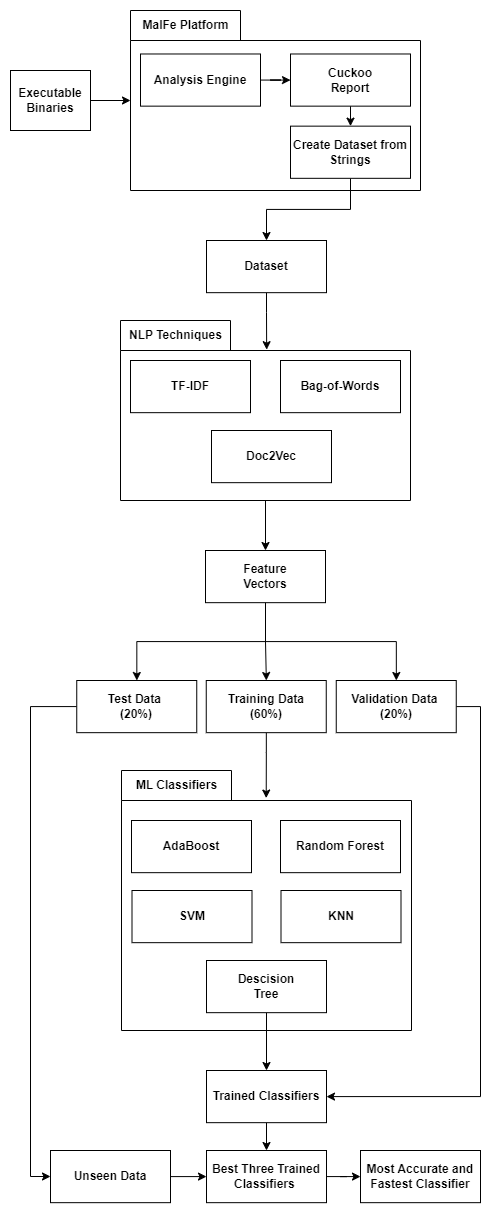
\includegraphics[scale=0.40]{Model.png}} \\
    \caption{Process Model}
    \label{fig:pModel}
\end{figure}


\subsection{NLP Techniques}
NLP techniques are a way to convert a corpus of words into a real-valued vector in such a way that the semantics and relationships between the words are captured \cite{turing-nlp}. \par
In this research, the strings were extracted from Cuckoo sandbox reports from the MalFe platform \cite{malfe}. The strings of a file are extracted by finding matches with the two regular expressions, namely \textbf{b"[\textbackslash x1f-\textbackslash x7e]{6,}"} and \textbf{b"(?:[\textbackslash x1f-\textbackslash x7e][\textbackslash x00]){6,}"} \cite{cuckoo-strings}. The strings are then capped at a length of 1024 characters, and a maximum of 2048 strings are extracted from a file. Some examples of matched strings are: \textbf{"VWUUhP@@"}, \textbf{"The unexpected small block leaks are:"}, \textbf{"EInvalidOp"} and \textbf{"Inno Setup Messages (5.5.0) (u)"}. \\

\subsubsection{Term Frequency-Inverse Document Frequency}
TF-IDF is an NLP technique that considers the frequency of the appearance of a word in a document and divides this by the number of documents in the corpus that the word appears in. It can be formulated as follows:
\begin{equation*}
\begin{array}{l}
TF = \frac{\textnormal{number of times the term appears in the document}}{\textnormal{total number of terms in the document}} \\\\
IDF = log(\frac{\textnormal{number of the documents in the corpus}}{\textnormal{number of documents in the corpus that contain the term}}) \\\\
TF-IDF = TF*IDF
\end{array}
\end{equation*}

Thus, it measures how important a word is within a specific document \cite{tf-idf}. So as an example, consider a corpus of three documents:\\
\textbf{\textit{Document 1: 'data science is one of the most important fields of science'\\
Document 2: 'this is one of the best data science courses'\\
Document 3: 'data scientists analyze data'\\}}
In the first document, the first word is 'data', since the word appears once in the document and there are 11 words in total in the document, the $TF = \frac{1}{11} = 0.090909$. Then, since there are 3 documents in the corpus and the term 'data' appears in all three, $IDF = log(\frac{3}{3}) = 0$, thus the TF-IDF term for the term 'data' in the first document would be $0.090909*0 = 0$. Calculating this for each of the terms in the corpus with respect to the first document would yield the vector representation: $[$0.043375, 0.00000, 0.000000, 0.000000, 0.000000, 0.00000, 0.032017, 0.043375, 0.016008, 0.016008, 0.032017, 0.043375, 0.016008, 0.0$]$. This process can then be completed for each of the other documents in the corpus to get a vector of three vectors, each of the same length as the total number of unique words in the corpus.\\

\subsubsection{Bag-of-words}
Bag-of-words is an NLP technique representing each document in the corpus as a vector of a fixed length, equal to the total vocabulary size. If the word corresponding to the index in the vector is present in the document, it is represented by a one (1); otherwise, it is represented by a zero (0) \cite{bag-of-words}. As an example, consider a corpus of four documents as follows:\\
\textbf{\textit{Document 1: 'It was the best of times'\\
Document 2: 'it was the worst of times'\\
Document 3: 'it was the age of wisdom'\\
Document 4: 'it was the age of foolishness'\\}}
Next, take all of the unique words in any order, for example: “it”, “was”, “the”, “best”, “of”, “times”, "worst”, “age”, “wisdom” and “foolishness”. The first document would then have a vector representation of: $[$1, 1, 1, 1, 1, 1, 0, 0, 0, 0$]$ since the first five words in the list of unique words in the corpus appear in the document, while the last four do not \cite{bow-example}.\\

\subsubsection{Doc2Vec}
Doc2Vec is an NLP technique that extends the popular Word2vec NLP technique by adding a paragraph vector. Thus, instead of creating a vector of a word, it encodes an entire document into a vector \cite{doc2vec}. Word2Vec works by training a simple neural network with a single hidden layer on the corpus of data; the embedding that is then created in the hidden layer can then be used as a representation of the corpus. Doc2Vec extends this by adding another paragraph ID vector that is unique to each document. These two vectors are then concatenated which results in the final vector representation of each of the documents in the corpus \cite{doc2vec-explained}. Since the number of neurons in the hidden layers of the neural networks can be controlled, the size of the vector representation can be controlled. As an example, if we take the corpus:\\
\textit{\textbf{Document 1: 'Come end of fall, the winds will grow' \\
Document 2: 'then twisting branches will cusp the snow' \\
Document 3: 'but spring will free what cold held dear'\\ 
Document 4: 'give way, give way, for one more year'\\}}
The Doc2Vec representation of the first document with a vector size of 10 would be $[$-0.04018994, 0.0330957, 0.02324159, -0.0238918, -0.0057377, 0.02368324, -0.02787386, -0.02250209, 0.04231475, 0.01566228$]$

\subsection{Dataset}
\urldef{\dataset}\url{https://malfe.cs.up.ac.za/datasets/view/RDS/60#version1}
% Go into more detail about what the dataset consists of and some other stats about it
The data consisted of 3325 executable files of which 1497 files are benign, and 1828 are malicious. These executable samples were sourced from TheZoo, PortableApps, DikeDataset and MalwareBazaar. These strings were extracted from raw Cuckoo Sandbox reports using the MalFe platform \cite{malfe}. The raw dataset can be found with the name "Ransomware Detection Using Strings"\footnote{\dataset} on the MalFe platform. The distribution of the categories of data is demonstrated in Table \ref{tab:datasetCat}. In total, the files contained millions of strings, with an average of 1501 strings per file. The executable files strings contain valuable information about the executable and, as such, they are treated as natural language strings. This allows for positional and relational information about the strings to be encoded and increases the efficacy of the ML techniques. The next step is to pre-process this data by feeding it into NLP techniques. 
\begin{table}[H]
 \begin{center}
 \caption{\label{tab:datasetCat} Dataset Categories.}
\begin{tabular}{|c|c|}
 \hline
\textbf{Category} & \textbf{Count} \\\hline 
Ransomware       & 1828 \\\hline
Utilities        & 223 \\\hline
Internet         & 86 \\\hline
Graphics         & 55 \\\hline
Office           & 54 \\\hline
Games            & 52 \\\hline
Music / Video    & 46 \\\hline
Security         & 30 \\\hline
Development      & 20 \\\hline
Education        &  9 \\\hline
Benign (Other)   & 970 \\\hline
\end{tabular}
 \end{center}

\end{table}

\subsection{Data Quality and Statistics}
Printable strings were extracted statically from each binary and aggregated per sample. The average string length per sample differs substantially between classes:
\begin{itemize}
    \item Benign samples: mean average string length of 2453 characters
    \item Ransomware samples: mean average string length of 4224 characters
\end{itemize}

This difference suggests that ransomware binaries tend to embed longer printable string sequences, which may include encrypted payload fragments, embedded resources, or statically linked metadata. Importantly, this observation reflects string length, not string count, indicating that ransomware often contains fewer but substantially longer printable regions. The number of long strings (defined as strings exceeding 20 characters) also varies between classes. Benign samples exhibit a higher mean count of long strings (42 per sample) compared to ransomware (27 per sample). This indicates that benign software tends to include numerous medium-length, human-readable strings (e.g., API names, file paths, UI text), whereas ransomware strings are more skewed toward fewer, very long sequences.\\

To assess the semantic quality of extracted strings, Shannon entropy was computed per string and averaged per sample. The results show comparable entropy levels across classes:
\begin{itemize}
    \item Benign: mean entropy 4.71
    \item Ransomware: mean entropy 4.56
\end{itemize}
Both classes fall within a mid-entropy regime, indicating that the dataset is not dominated by either low-entropy boilerplate text or high-entropy encrypted noise. The slightly lower entropy observed in ransomware strings suggests the presence of structured, repetitive content (e.g., manifest metadata, API names, privilege requests) alongside obfuscated regions. These results confirm that the extracted printable strings retain meaningful semantic structure, supporting their suitability for downstream statistical and machine-learning analysis.\\

To evaluate robustness to noise and low-information strings, strings shorter than increasing minimum lengths were progressively removed. The average number of retained strings per sample decreases smoothly with stricter thresholds for both classes:
\begin{itemize}
    \item With a minimum length of 4 characters, benign samples retain 49 strings on average, compared to 37 for ransomware.
    \item At a minimum length of 16 characters, benign samples retain 44 strings, while ransomware retain 28.
\end{itemize}
The monotonic and gradual decline indicates that the dataset does not rely on a small number of short, fragile indicators. Instead, discriminative information persists even after aggressive pruning, suggesting that the printable strings exhibit robust signal density rather than brittle keyword dependence.\\

To quantify the informativeness of individual strings, mutual information (MI) was computed between binary string presence and the ransomware label. Highly ranked strings include:
\begin{itemize}
    \item Structural PE sections (e.g., .data, .rdata)
    \item Windows API references (e.g., kernel32.dll, GetLastError)
    \item Application manifests and privilege descriptors (e.g., requestedExecutionLevel, trustInfo)
    \item Configuration and metadata terms (e.g., assembly, manifestVersion, security)
\end{itemize}
The diversity of high-MI strings indicates that discrimination is not driven by a single keyword or artefact, but rather by a broad spectrum of semantically meaningful indicators spanning binary structure, execution privileges, and system interaction. The top 20 strings are presented in Table \ref{tab:mi}
\begin{table}[H]
\begin{center}
    \caption{\label{tab:mi} MI of top 20 strings.}
    \begin{tabular}{|l|l|}
     \hline
    \textbf{String}         & \textbf{MI}   \\ \hline
    version                 & 0.599293      \\ \hline
    .data                   & 0.562157      \\ \hline
    kernel32.dll            & 0.542670      \\ \hline
    name                    & 0.542467      \\ \hline
    .rdata                  & 0.501461      \\ \hline
    assembly                & 0.488292      \\ \hline
    type                    & 0.483308      \\ \hline
    security                & 0.481017      \\ \hline
    level                   & 0.476413      \\ \hline
    getcurrentprocess       & 0.471400      \\ \hline
    xmlns                   & 0.470347      \\ \hline
    false                   & 0.466049      \\ \hline
    schemas-microsoft-com   & 0.464501      \\ \hline
    manifestversion         & 0.464119      \\ \hline
    asm.v1                  & 0.463737      \\ \hline
    getlasterror            & 0.461255      \\ \hline
    trustinfo               & 0.458204      \\ \hline
    requestedprivileges     & 0.457824      \\ \hline
    requestedexecutionlevel & 0.457824      \\ \hline
    system                  & 0.454032      \\ \hline
    \end{tabular}
\end{center}
\end{table}
Overall, the dataset exhibits several desirable quality properties:
\begin{itemize}
    \item Balanced and heterogeneous class composition, reducing sampling bias.
    \item Non-trivial string length and entropy distributions, indicating meaningful printable content.
    \item Robustness to string pruning, suggesting resilience to noise and obfuscation.
    \item A long tail of informative strings, rather than reliance on a small number of signatures.
\end{itemize}
These characteristics support the use of printable strings as a reliable and interpretable feature source for ransomware detection and justify their evaluation in subsequent classification experiments.

\subsection{Data Pre-processing}
The extracted strings were converted into feature vectors using three NLP techniques: TF-IDF, Bag-of-Words and Doc2Vec. 
TF-IDF converted the corpus of strings of all the executables into a 2D matrix with 1479647 features representing each input document. Bag-of-Words converts the corpus into a 2D matrix with 664140 features representing each document. Doc2Vec is trained on the input data and can produce a vector of any specified length to represent an executable's strings. An array length of 1000 was used. Now that the NLP techniques were applied separately to the dataset essentially providing a dataset for each technique. Each dataset was then split into 60\% training, 20\% validation, and 20\% testing. The details of the dataset split and features are shown in Table \ref{tab:dataset}. This dataset is heavily imbalanced, however, this was due to the limited benign samples that the platform had \cite{malfe}. 
 
\begin{table}[H]
\caption{\label{tab:dataset} NLP data metrics.}
\resizebox{9cm}{!}{
\begin{tabular}{|l|l|l|l|}
\hline
 
 & Bag-of-Words & TF-IDF & Doc2Vec \\ \hline
Features & 804801 &  1711443 & 1000\\ \hline
Fit time (min) &  0.1260 & 0.1670 & 7.9008  \\ \hline
Training Length  & 2026 & 2026 & 2026\\ \hline
Training Malicious  & 1098 &  1098 & 1098\\ \hline
Training Benign  & 928 &  928 & 928\\ \hline
Validation Length & 675 & 675 & 675\\ \hline
Validation Malicious  & 366 &  366 & 366\\ \hline
Validation Benign  & 309 &  309 & 309\\ \hline
Test Length & 676 & 676 & 676\\ \hline
Test Malicious  & 366 & 366 & 366\\ \hline
Test Benign  & 310 &  310 & 310\\ \hline
\end{tabular}
}
\end{table}

  
 

\subsection{Machine Learning Classifiers}
The feature vectors from the pre-processors are then fed into ML classifiers for training. The five (5) ML classifiers selected are Decision Tree (DT), Random Forest (RF), AdaBoost (AB), Support Vector Machine (SVM), and K-Nearest-Neighbours (KNN). These classifiers were selected due to the nature of the dataset as well as for their performance in terms of training and prediction times. The goal is to have fast training and prediction times such that the classifier can be deployed in a real-world environment. Therefore, RF and DT were chosen to make sense of the data through rule-based deductions. Boosted learning, such as AB, was also explored to see if more deductions can be made by evolving the classifier over a number of iterations. SVM and KNN were also considered to see if hyperplanes or clustering could perform better. All the training of the ML classifiers underwent hyperparameter tuning as well as five-fold cross-validation. This was done to ensure the best model parameters were chosen, as well as to ensure there is no bias and noise in the model by performing cross-validation. A variety of metrics were used to evaluate the performance of the system, such as True Positive(TP), False Positive (FP), True Negative (TN), False Negative (FN), Recall, Precision, F1-score, Accuracy, Area Under the Curve (AUC), logloss and latency. The AUC and logloss, on the other hand, define the models correctness and confidence in its prediction. Finally, the latency is the time taken to perform the prediction for the specified model. The source code, results and processed dataset are available at the RDS GitHub repository \cite{Daneel2022}.  \\

\subsubsection{Decision Tree}
The Decision Tree (DT) classifier is a model that classifies data points using a series of if-else rules organized in a tree structure. It is easy to understand and interpret due to its visual nature. Additionally, DTs typically perform well with minimal data preprocessing. The best-performing configuration was achieved using the Bag-of-Words representation, with the parameters \texttt{criterion='log\_loss'} and \texttt{splitter='best'}. Among all preprocessing methods, TF-IDF produced the highest accuracy of 94.96\% and the lowest false positives and false negatives, indicating it was the most effective configuration overall (see Table~\ref{tab:table-dt2}). The default values were used for all other parameters.

\begin{table}[H]
\caption{\label{tab:table-dt} Metrics for the Decision Tree Classifier.}
\resizebox{9cm}{!}{
\begin{tabular}{|l|l|l|l|l|l|l|l|}
\hline
 & TP & TN & FP & FN & Recall & Precision & F1-Score \\ \hline
Bag-of-Words & 293 & 348 & 18 & 16 & 0.9508 & 0.956 & 0.9534 \\ \hline
TF-IDF & 293 & 348 & 18 & 16 & 0.9508 & 0.956 & 0.9534  \\ \hline
Doc2Vec & 208 & 266 & 100 & 101 & 0.7268 & 0.7248 & 0.7258 \\ \hline
\end{tabular}
}
\end{table}
\vspace{-1.5ex}
\begin{table}[H]
\caption{\label{tab:table-dt2} Performance Metrics for the Decision Tree Classifier.}
\resizebox{9cm}{!}{
\begin{tabular}{|l|l|l|l|l|p{1.5cm}|}
\hline
 & Accuracy & AUC & Log Loss & Latency(ms) & Average Latency Per Sample (ms) \\ \hline
Bag-of-Words & 0.9496 & 0.9495 & 1.8155 & 27.5192 & 0.0408 \\ \hline
TF-IDF   & 0.9496 & 0.9495 & 1.8155 & 33.2804 & 0.0493  \\ \hline
Doc2Vec  & 0.7022 & 0.7 & 10.733 & 1.1332 & 0.0017  \\ \hline
\end{tabular}
}
\end{table}
 
\subsubsection{Random Forest}
The Random Forest (RF) classifier is a meta-estimator that builds multiple decision trees on random subsets of the training data and aggregates their predictions to improve accuracy and reduce overfitting. The best-performing configuration was achieved using the Bag-of-Words representation, with \texttt{max\_depth = 8} and \texttt{n\_estimators = 5}, yielding a mean test score of 0.9917 and a standard deviation of 0.0104. As shown in Table~\ref{tab:table-rf2}, the Bag-of-Words approach achieved the highest accuracy of 99.16\%, with zero false positives and a fast prediction time of 0.1932ms. All other hyperparameters were set to their default values.


\begin{table}[H]
\caption{\label{tab:table-rf} Metrics for the Random Forrest Classifier.}
\resizebox{9cm}{!}{
\begin{tabular}{|l|l|l|l|l|l|l|l|}
\hline
 & TP & TN & FP & FN & Recall & Precision & F1-Score \\ \hline
Bag-of-Words &  295 & 356 & 10 & 14 & 0.9727 & 0.9622 & 0.9674  \\ \hline
TF-IDF &  295 & 357 & 9 & 14 & 0.9754 & 0.9623 & 0.9688 \\ \hline
Doc2Vec & 252 & 311 & 55 & 57 & 0.8497 & 0.8451 & 0.8474 \\\hline
\end{tabular}
}

\end{table}
\vspace{-1.5ex}
\begin{table}[H]
\caption{\label{tab:table-rf2} Performance Metrics for the Random Forrest Classifier.}
\resizebox{9cm}{!}{
\begin{tabular}{|l|l|l|l|l|p{1.5cm}|}
\hline
 & Accuracy & AUC & Log Loss & Latency(ms) & Average Latency Per Sample (ms) \\ \hline
Bag-of-Words & 0.9644 & 0.9949 & 0.1211 & 288.6295 & 0.4276 \\ \hline
TF-IDF   & 0.9659 & 0.9959 & 0.105 & 2331.629 & 3.4543  \\ \hline
Doc2Vec  & 0.8341 & 0.913 & 0.4363 & 22.3072 & 0.033 \\\hline
\end{tabular}
}
\end{table}

\subsubsection{AdaBoost}
The AdaBoost (AB) classifier is a meta-estimator that initially trains a base classifier and iteratively fits additional classifiers to better handle difficult cases. The best performance was achieved using the TF-IDF representation with parameters \texttt{learning\_rate = 0.1} and \texttt{n\_estimators = 250}. This configuration attained a mean test score of 0.9937 and a standard deviation of 0.0081. As shown in Table~\ref{tab:table-ada2}, TF-IDF achieved over 99\% in both recall and accuracy, but exhibited high latency, requiring 8.9791ms to classify a single sample. All other hyperparameters were kept at their default values.


\begin{table}[H]
\caption{\label{tab:table-ada} Metrics for the AdaBoost Classifier.}
\resizebox{9cm}{!}{
\begin{tabular}{|l|l|l|l|l|l|l|l|}
\hline
 & TP & TN & FP & FN & Recall & Precision & F1-Score \\ \hline
Bag-of-Words & 295 & 356 & 10 & 14 & 0.9727 & 0.9622 & 0.9674   \\ \hline
TF-IDF &  297 & 359 & 7 & 12 & 0.9809 & 0.9677 & 0.9742   \\ \hline
Doc2Vec & 232 & 305 & 61 & 77 & 0.8333 & 0.7984 & 0.8155\\ \hline
\end{tabular}
}
\end{table}

\begin{table}[H]
\caption{\label{tab:table-ada2} Performance Metrics for the AdaBoost Classifier.}
\resizebox{9cm}{!}{
\begin{tabular}{|l|l|l|l|l|p{1.5cm}|}
\hline
 & Accuracy & AUC & Log Loss & Latency(ms) & Average Latency Per Sample (ms) \\ \hline
Bag-of-Words &  0.9644 & 0.9942 & 0.5731 & 7054.8534 & 10.4516 \\ \hline
TF-IDF   &  0.9719 & 0.9927 & 0.5748 & 10956.3744 & 16.2317  \\ \hline
Doc2Vec  & 0.7956 & 0.8788 & 0.6408 & 117.5032 & 0.1741 \\ \hline
\end{tabular}
}
\end{table}

\subsubsection{SVM}
Support Vector Machines (SVM) are supervised learning models that perform well in high-dimensional spaces and remain effective even when the number of samples is smaller than the number of features. The best results were obtained using the TF-IDF representation with parameters \texttt{C = 10} and \texttt{kernel = 'sigmoid'}, achieving a mean test score of 0.9917 and a standard deviation of 0.0083. As shown in Table~\ref{tab:table-svm2}, this configuration yielded an accuracy above 99\% and maintained high recall and low false positives. All other hyperparameters were set to their default values.


\begin{table}[H]
\caption{\label{tab:table-svm} Metrics for the SVM Classifier.}
\resizebox{9cm}{!}{
\begin{tabular}{|l|l|l|l|l|l|l|l|}
\hline
 & TP & TN & FP & FN & Recall & Precision & F1-Score \\ \hline
Bag-of-Words &  296 & 354 & 12 & 13 & 0.9672 & 0.9646 & 0.9659    \\ \hline
TF-IDF &   288 & 360 & 6 & 21 & 0.9836 & 0.9449 & 0.9639    \\ \hline
Doc2Vec & 195 & 298 & 68 & 114 & 0.8142 & 0.7233 & 0.7661 \\\hline
\end{tabular}
}

\end{table}

\begin{table}[H]
\caption{\label{tab:table-svm2} Performance Metrics for the SVM Classifier.}
\resizebox{9cm}{!}{
\begin{tabular}{|l|l|l|l|l|p{1.5cm}|}
\hline
 & Accuracy & AUC & Log Loss & Latency(ms) & Average Latency Per Sample (ms) \\ \hline
Bag-of-Words &  0.963 & 0.9855 & 0.1376 & 2480.1817 & 3.6743 \\ \hline
TF-IDF   &  0.96 & 0.9884 & 0.1502 & 6381.0563 & 9.4534  \\ \hline
Doc2Vec  &  0.7304 & 0.802 & 0.5541 & 331.9006 & 0.4917  \\\hline
\end{tabular}
}
\end{table}

\subsubsection{K-Nearest Neighbors}
K-Nearest Neighbours (KNN) is a non-generalizing learning algorithm that classifies samples based on a majority vote of the \(k\) nearest neighbours, where \(k\) is a user-defined parameter. The best performance was achieved with the TF-IDF representation using parameters \texttt{leaf\_size = 5}, \texttt{n\_neighbors = 5}, \texttt{p = 2}, and \texttt{weights = 'distance'}, yielding a mean test score of 0.9868 and a standard deviation of 0.0142. As shown in Table~\ref{tab:table-knn2}, despite achieving relatively high accuracy with TF-IDF, KNN exhibited the poorest overall performance among the classifiers, particularly with the Doc2Vec preprocessor, which resulted in an accuracy of just 82.25\%. Additionally, KNN had consistently high false positive rates and the highest prediction latency, taking over 355ms per sample. All other hyperparameters were left at their default values.


\begin{table}[H]
\caption{\label{tab:table-knn} Metrics for the KNN Classifier.}
\resizebox{9cm}{!}{
\begin{tabular}{|l|l|l|l|l|l|l|l|}
\hline
 & TP & TN & FP & FN & Recall & Precision & F1-Score \\ \hline
Bag-of-Words &  266 & 355 & 11 & 43 & 0.9699 & 0.892 & 0.9293   \\ \hline
TF-IDF &   294 & 340 & 26 & 15 & 0.929 & 0.9577 & 0.9431   \\ \hline
Doc2Vec &  206 & 309 & 57 & 103 & 0.8443 & 0.75 & 0.7943 \\ \hline
\end{tabular}
}
\end{table}

\begin{table}[H]
\caption{\label{tab:table-knn2} Performance Metrics for the KNN Classifier.}
\resizebox{9cm}{!}{
\begin{tabular}{|l|l|l|l|l|p{1.5cm}|}
\hline
 & Accuracy & AUC & Log Loss & Latency(ms) & Average Latency Per Sample (ms) \\ \hline
Bag-of-Words & 0.92 & 0.9732 & 0.7809 & 796.4272 & 1.1799 \\ \hline
TF-IDF   &  0.9393 & 0.9741 & 0.7791 & 438.1878 & 0.6492  \\ \hline
Doc2Vec  &  0.763 & 0.8519 & 1.8379 & 1776.0074 & 2.6311 \\\hline
\end{tabular}
}
\end{table}

\section{Reinforcement Learning Extension}
We extended the supervised strings pipeline with a compact reinforcement-learning (RL) experiment to investigate whether a small policy can be bootstrapped from a high-performing supervised detector and subsequently adapted by interaction. The primary aims were: (1) provide a reproducible recipe to convert a static detector into a lightweight policy suitable for online refinement; and (2) evaluate the practical gains and trade-offs of such an approach on the RDS dataset.

\subsection{Environment and reward design}
To keep the initial experiment simple and interpretable we framed the dataset as a deterministic, episodic environment. Each episode iterates once through the training split in a fixed order; at each step the agent receives the TF-IDF feature vector for a single file and must return an action $a\in\{0,1\}$ that corresponds to the predicted label. We use an immediate reward of $+1$ for a correct label and $-1$ for an incorrect label. The deterministic traversal reduces environmental variance due to stochastic sampling and isolates policy improvement dynamics.

The reward is intentionally symmetric and sparse (binary correctness) which keeps credit assignment straightforward and aligns the RL objective with supervised accuracy while still allowing policy-gradient updates to shift behaviour based on cumulative episode returns.

\subsection{Policy architecture and pretraining}
The policy is a small multilayer perceptron: an input linear layer (dimension = TF-IDF feature length) to a hidden layer of 128 ReLU units, followed by a linear output layer producing two logits. A softmax converts logits into a categorical distribution over actions. The small capacity is chosen to keep inference fast and to reduce overfitting risk on the relatively small training split.

Before running RL updates we perform behavioural cloning: we select the best supervised model on validation (see Table~\ref{tab:val-models}) and use it to label the training split. The policy is trained for a small number of epochs (5) with CrossEntropy loss to imitate the teacher. This step provides a strong, high-precision initialization, substantially reducing early random exploration and stabilising policy-gradient updates.

\subsection{Policy-gradient fine-tuning (REINFORCE)}
We apply an episodic REINFORCE update loop. Each episode collects log-probabilities of sampled actions and the scalar rewards for each time-step. Returns are computed with discount factor $\gamma$; to reduce variance we normalise the per-episode returns to zero mean and unit variance prior to computing policy gradients. The per-step policy loss is the negative log-probability multiplied by the corresponding normalised return; gradients are accumulated over the episode and applied with the Adam optimiser (lr = $1\times10^{-3}$). In our experiments we used $\gamma=0.99$ and 30 episodes.

Normalising returns acts as a simple baseline and reduces the impact of scale differences between episodes; combined with the behaviour-cloning initialization this reduces gradient variance and helps avoid mode collapse or catastrophic policy shifts. The deterministic environment also prevents variance caused by random sampling order.

\subsection{Mitigating bias and overfitting}
We took several pragmatic steps to reduce bias introduced by the RL procedure and to make evaluation fair and comparable to the supervised baseline:
\begin{itemize}
  \item Model selection for behavioural cloning uses validation F1 (not training loss), ensuring the teacher model generalises to held-out data before bootstrapping the policy.
  \item Behavioural cloning is run for a small, fixed number of epochs (5) to imitate teacher behaviour without fully memorising noisy labels.
  \item Per-episode normalisation of returns reduces episodic scale differences and prevents large-magnitude gradients dominated by a few episodes.
  \item The final policy is evaluated only on the held-out test split (never used during selection or RL updates) to provide an unbiased performance estimate.
\end{itemize}

These measures do not eliminate all sources of bias (for instance, the teacher's mistakes can be transferred to the policy), but they significantly constrain overfitting and ensure the RL steps act as a refinement rather than an unconstrained re-training.

\subsection{Validation-stage model comparison}
Before bootstrapping, we evaluated all candidate supervised models on the validation split and selected the highest-F1 model (AdaBoost on TF-IDF). Table~\ref{tab:val-models} summarises the validation F1 scores for the models considered (extracted from the experiment logs).

\begin{table}[h!]
\caption{Validation F1 scores for candidate supervised models (selection stage).}
\label{tab:val-models}
\resizebox{9cm}{!}{
\begin{tabular}{|l|l|}
\hline
Model & Validation F1 \\
\hline
AB\_TFIDF & 0.97422 \\
AB\_BOW & 0.96739 \\
RF\_TFIDF & 0.96879 \\
RF\_BOW & 0.96739 \\
SVM\_TFIDF & 0.96386 \\
SVM\_BOW & 0.96589 \\
DT\_TFIDF & 0.95342 \\
DT\_BOW & 0.95342 \\
KNN\_TFIDF & 0.94313 \\
KNN\_BOW & 0.92932 \\
RF\_DOC2VEC & 0.84741 \\
AB\_DOC2VEC & 0.81551 \\
KNN\_DOC2VEC & 0.79434 \\
SVM\_DOC2VEC & 0.76607 \\
DT\_DOC2VEC & 0.72578 \\
\hline
\end{tabular}
}
\end{table}

\subsection{RL experimental results}
After behavioural cloning and REINFORCE fine-tuning (30 episodes) we evaluated the learned policy on the held-out test split. Table~\ref{tab:rl-metrics} reproduces the classification report extracted from the test run.

\begin{table}[h!]
\caption{RL policy test metrics (classification report).}
\label{tab:rl-metrics}
\resizebox{9cm}{!}{
\begin{tabular}{|l|c|c|c|c|}
\hline
Class & Precision & Recall & F1-score & Support \\
\hline
0 (Benign) & 0.90 & 0.95 & 0.93 & 310 \\
1 (Ransomware) & 0.95 & 0.92 & 0.93 & 366 \\
\hline
Accuracy & \multicolumn{4}{c|}{0.93} \\
Macro avg & 0.93 & 0.93 & 0.93 & 676 \\
Weighted avg & 0.93 & 0.93 & 0.93 & 676 \\
\hline
\end{tabular}
}
\end{table}

Figure~\ref{fig:rl-reward} is a placeholder for the RL training curve (episode return or average reward per episode). In our implementation the REINFORCE loop records per-episode cumulative reward and the behavioural-cloning loss; plotting these signals helps visualise convergence and stability. We include placeholders so the figures can be generated after re-running the training loop with logging enabled.

\begin{figure}[h!]
    \centering
    \includegraphics[scale=0.5]{plots/rl_reward_curve.png} \\
    \caption{RL training: cumulative reward per episode (placeholder).}
    \label{fig:rl-reward}
\end{figure}

\begin{figure}[h!]
    \centering
    \includegraphics[scale=0.5]{plots/rl_behavioral_loss.png} \\
    \caption{Behavioural cloning training loss (placeholder).}
    \label{fig:rl-loss}
\end{figure}

The RL policy achieves a final test accuracy of 0.93 and macro F1 of 0.93. Compared to the best supervised TF-IDF detectors (validation F1 $\approx0.974$), the RL policy is slightly lower in static performance but provides an adaptable policy that can continue to learn from future interactions or delayed labels.

\subsection{Interpretation}
Two practical takeaways emerge from the experiment. First, behavioural cloning from a high-quality supervised teacher produces an initial policy that already captures most discriminative structure in the TF-IDF representation; the RL phase acts as a light refinement rather than wholesale re-training. Second, the simple REINFORCE updates (with returns normalisation) are sufficient to preserve high performance while keeping the architecture and training cost modest, making this approach feasible for constrained deployment scenarios where occasional online updates are desired.

\section{Discussion}

\section{Discussion}
Overall, using strings with NLP and ML techniques as a ransomware detection mechanism provides good detection capabilities. In addition, the proposed method provides quick detection of ransomware; however, the training time was significantly more due to hyper-parameter tuning as well as five-fold cross-validation. On average, using a cluster of 56 logical processors and 378GB RAM, training times were between 0.3 min - 20 min. Prediction times were performed on a standard machine with 8 logical processors delivering times of 25ms - 4000ms. These low training and classification times mean that the system is fast enough that it could be the underpinnings of a system that is deployed in the real world. Typically, prediction times are the priority whilst maintaining high accuracy in order for real-time detection. \\

The best-performing classifiers are AB with TF-IDF, SVM with BOW and DT with TF-IDF, with accuracies of 99.58\%, 99.37\% and 99.16\% respectively. However, AB with TF-IDF provides prediction times of 8.9791ms, making it worse than SVM and DT in this case. Therefore, the best classifier will be determined by the fastest and most accurate. These three classifiers were then further evaluated to determine the best-performing classifier by performing predictions on testing data to further determine their performance on unseen data. 
The results for the testing data predictions are demonstrated in table \ref{tab:tablebest}.

\begin{table}[h!]
\caption{\label{tab:tablebest} Testing Data Predictions Of The Three Best Performing Classifiers.}
\resizebox{9cm}{!}{
\begin{tabular}{|l|l|l|l|}
\hline
& AB with TF-IDF & SVM with BOW & DT with TF-IDF \\ \hline
TP & 113 & 113 & 113\\ \hline
TN & 365 & 364 & 364\\ \hline
FP & 1 & 2 & 2\\ \hline
FN & 1 & 1 & 1\\ \hline
Recall & 0.9973 & 0.9945 & 0.9945\\ \hline
Precision & 0.9973 & 0.9973 & 0.9973\\ \hline
F1-Score & 0.9973 & 0.9959 & 0.9959\\ \hline
AUC & 0.9996 & 0.9993 & 0.9929\\ \hline
Log Loss & 0.3488 & 0.0327 & 0.2253\\ \hline
Latency (ms) & 167.4294 & 1671.4294 & 17.5536\\ \hline
Average latency per sample (ms) & 8.6390 & 3.4821 & 0.0366\\ \hline
Accuracy & 0.9958 & 0.9938 & 0.9938\\ \hline

\end{tabular}
}
\end{table}
  

Therefore, from the results, AB with TF-IDF still had the highest accuracy but the slowest prediction times. SVM with BOW and DT with TF-IDF scored an accuracy of 99.38\%. Although, the AUC for SVM was slightly better, overall, the faster prediction time was the deciding factor. Therefore, the best classifier is DT with TF-IDF, with an average latency per sample of 0.0366ms. Low FN predictions are ideal since an FN prediction would potentially lead to a user installing ransomware on their system while thinking it to be benign. This is coupled with the fact that the DT classifier trained in 0.1442min, further cements it as the best classifier. Since the dataset was heavily imbalanced, a test was conducted to balance the ransomware samples at random. The results of this can be found in Appendix A. As expected, the results differed slightly by approximately 2\% in accuracy. However, the other metrics are close to the results obtained from the unbalanced dataset.\\

To visualize the diagnostic ability of the classifiers, the Receiver Operating Characteristic (ROC) curves were plotted for each of the NLP and ML techniques. The ROC curve illustrates an unbiased view of binary classifiers relative to one another, in terms of their performance at all of the classification thresholds. The closer the classifiers are to a right angle in the top right corner, the better their performance. In Figure \ref{fig:rocCurveTF}, TF-IDF was used as the NLP technique. All of the classifiers are tightly grouped, however, SVM performed slightly better than the other four classifiers. In addition, KNN performed the worst out of all of the classifiers.
In Figure \ref{fig:rocCurveBag}, the Bag-of-Words NLP technique was used. Once again, all of the classifiers are tightly grouped, with SVM once again performing better than all of the other classifiers. The KNN and the DT classifiers performed the worst in prediction confidence.
In Figure \ref{fig:rocCurveDoc}, the ROC for the Doc2Vec NLP technique is shown. With this preprocessor, the classifiers are much more spread and perform worse than the other two NLP techniques. The SVM classifier again performed the best, and DT performed the worst of all of the classifiers in the ROC.  \\ 

When compared with existing antivirus solutions such as VirusTotal and Microsoft Windows Defender, the proposed approach demonstrates improved generalisation to unseen ransomware samples. Conventional antivirus engines are primarily based on signature-driven techniques, where detection is performed through hash lookups, byte-pattern matching, or rule-based heuristics. These techniques are highly effective for known threats, but they struggle against zero-day variants or polymorphic ransomware, in which slight modifications to the binary are sufficient to bypass signature recognition. In contrast, the proposed method leverages the statistical and semantic properties of printable strings extracted from executables, thereby enabling the detection of variants that share linguistic or structural similarities even if they have not been previously observed. This provides an inherent advantage over strictly signature-based solutions. However, one of the main challenges lies in the use of obfuscation techniques, such as string encryption, packing, code morphing, or polymorphism, which can significantly reduce the presence of discriminative string features. In such cases, the effectiveness of NLP-based feature extraction is diminished. Nevertheless, it is important to note that complete removal or encryption of all meaningful strings imposes trade-offs for attackers. Executables that fully obfuscate string data typically exhibit high entropy characteristics, which are easily detectable through entropy-based heuristics or dynamic analysis techniques. Consequently, while obfuscation may degrade performance in a purely string-based classification setting, it often exposes the malware to detection by complementary static or behavioural mechanisms.

\begin{figure}[h!]
    \centering
    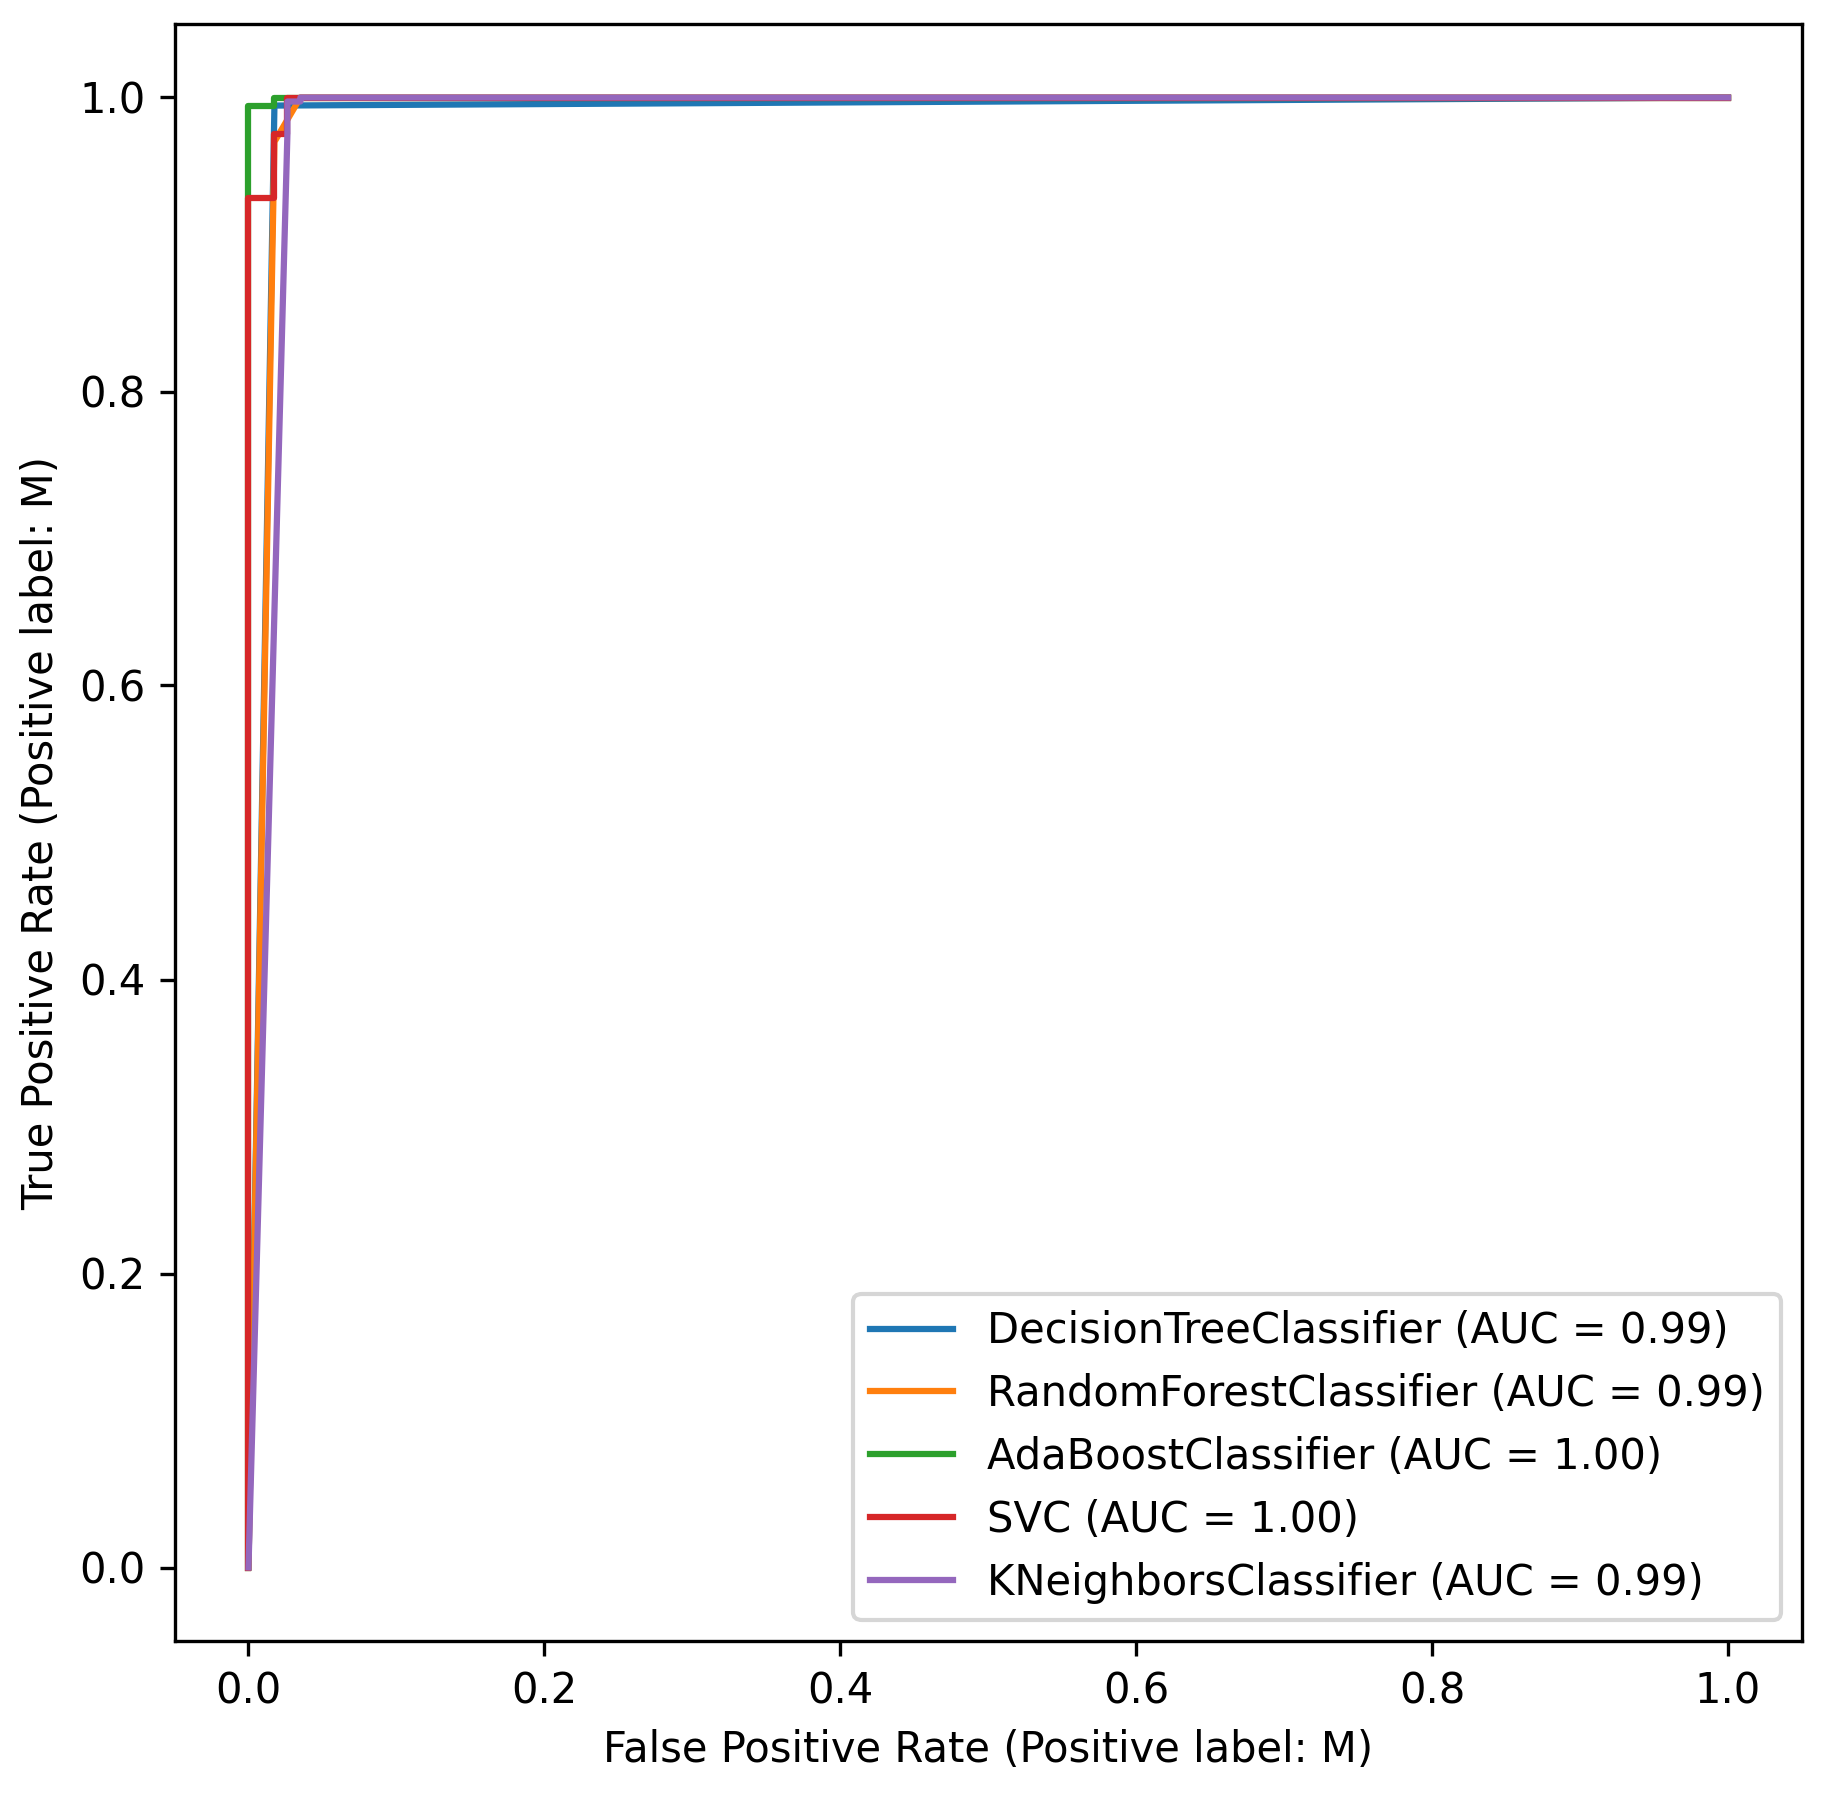
\includegraphics[scale=0.48]{plots/TFIDF.png} \\
    \caption{Roc Curve for TF-IDF}
    \label{fig:rocCurveTF}
\end{figure}

\begin{figure}[h!]
    \centering
    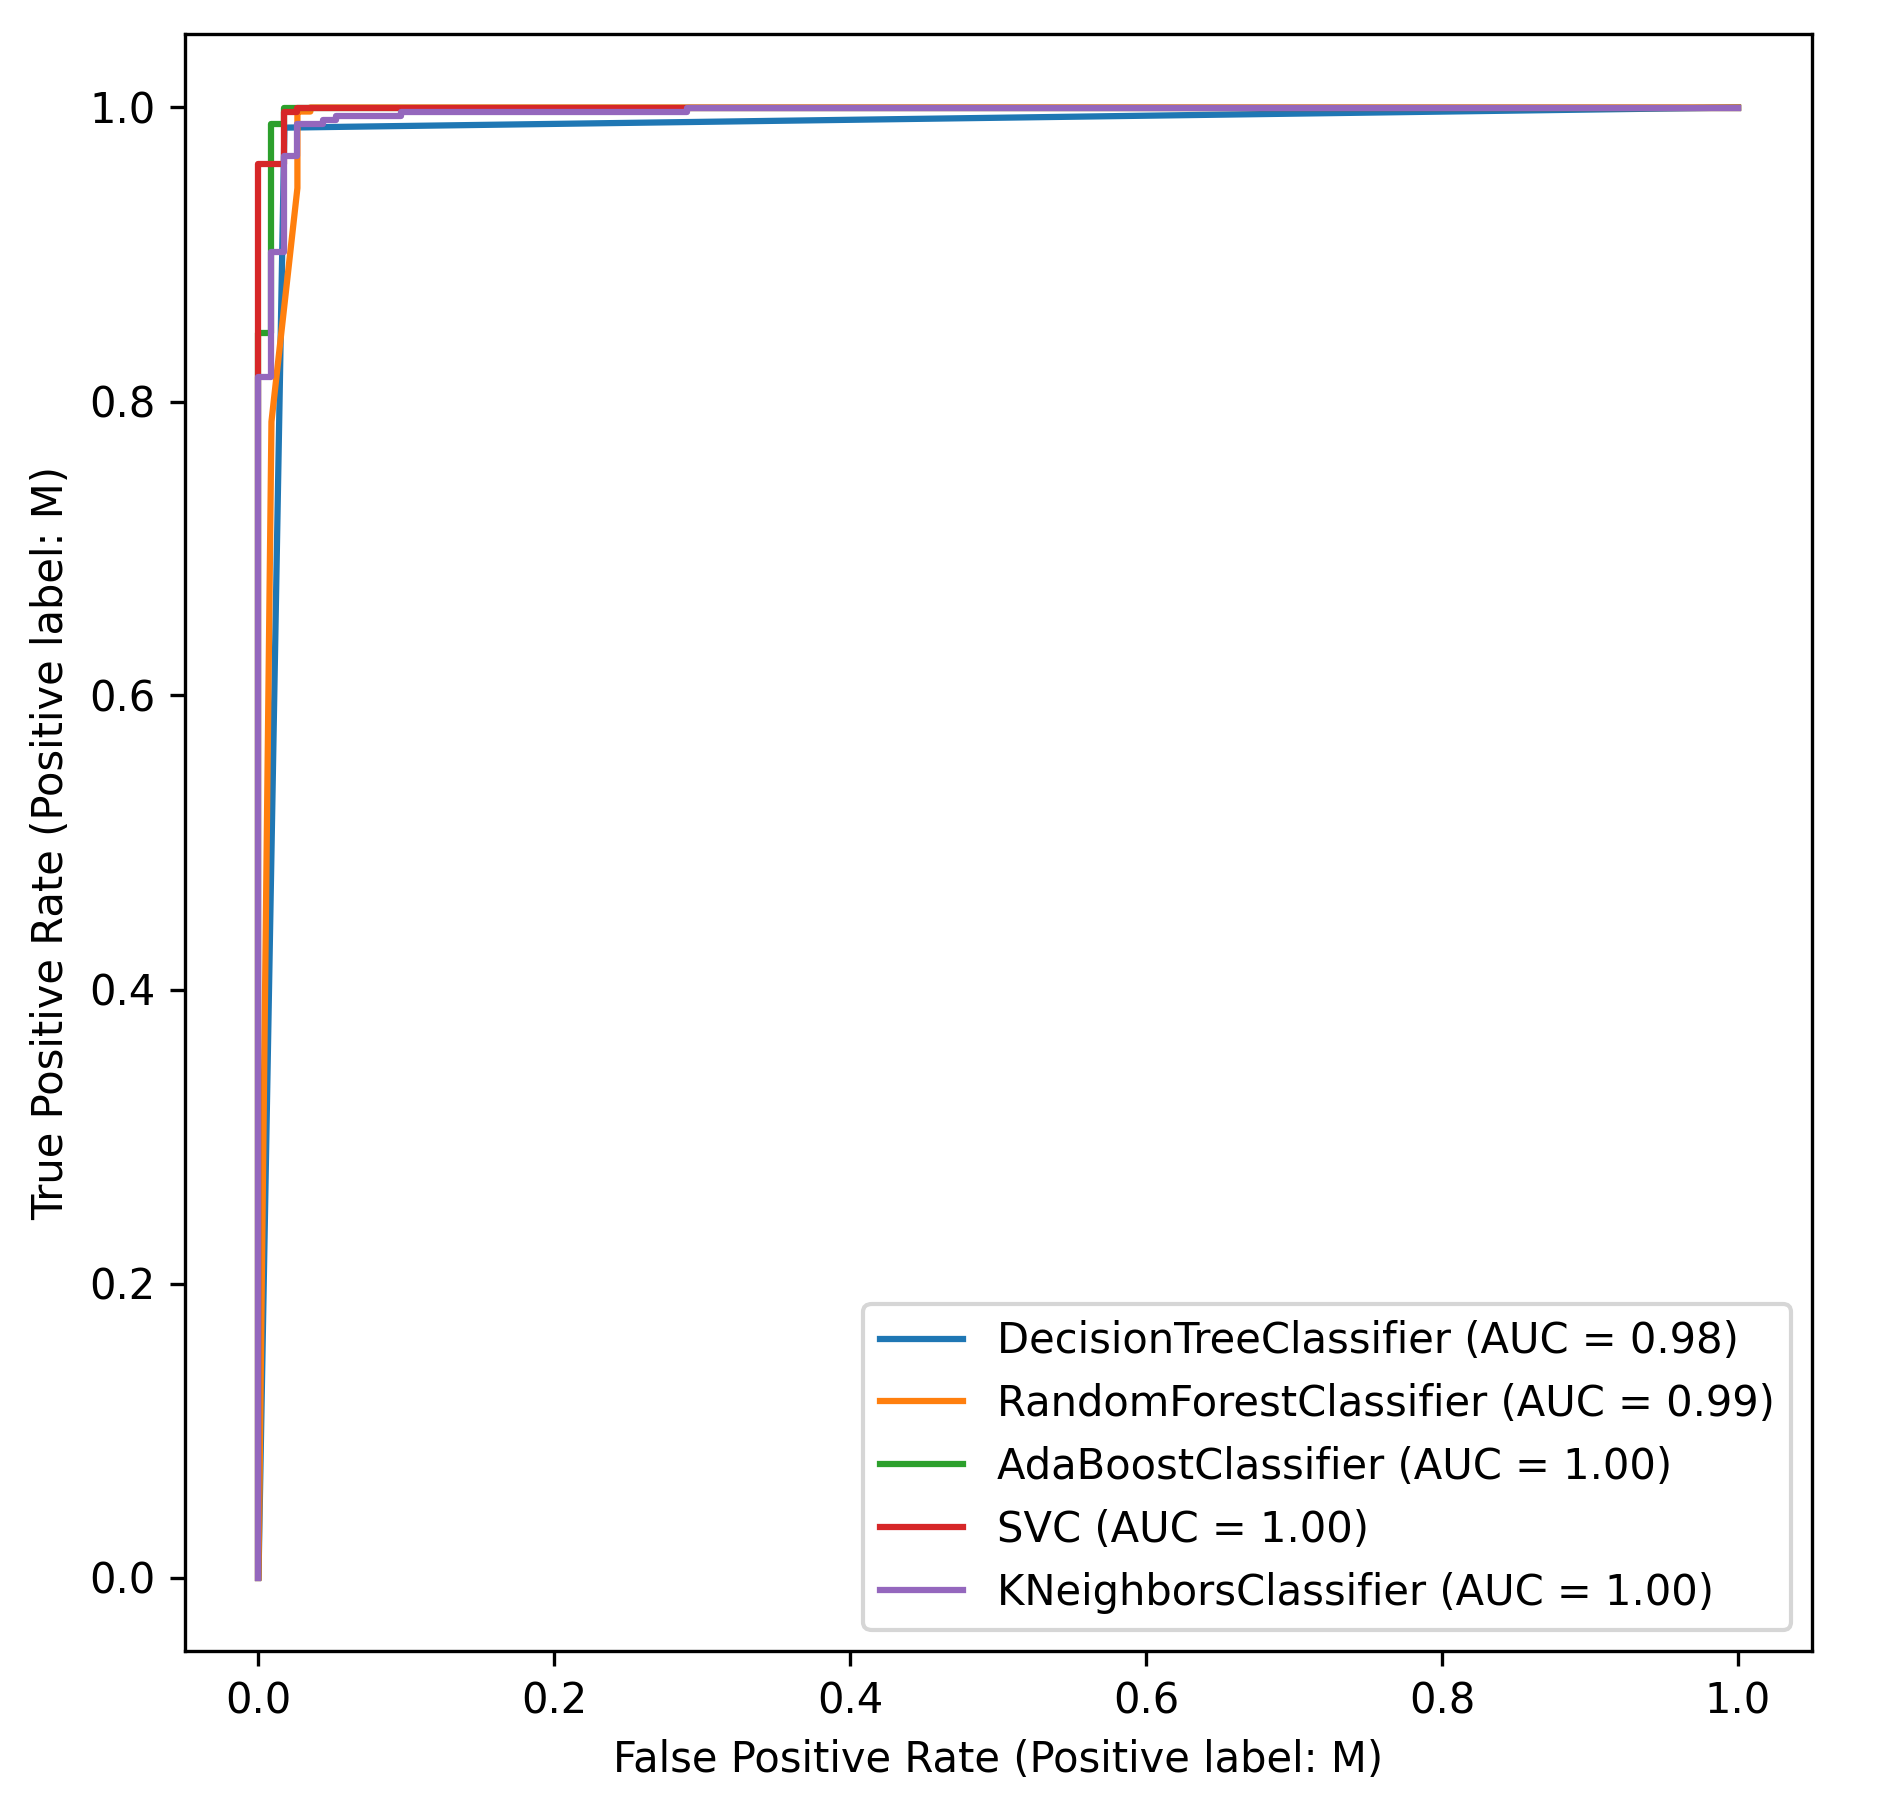
\includegraphics[scale=0.48]{plots/BOW.png} \\
    \caption{Roc Curve for Bag-of-Words}
    \label{fig:rocCurveBag}
\end{figure}

\begin{figure}[h!]
    \centering
    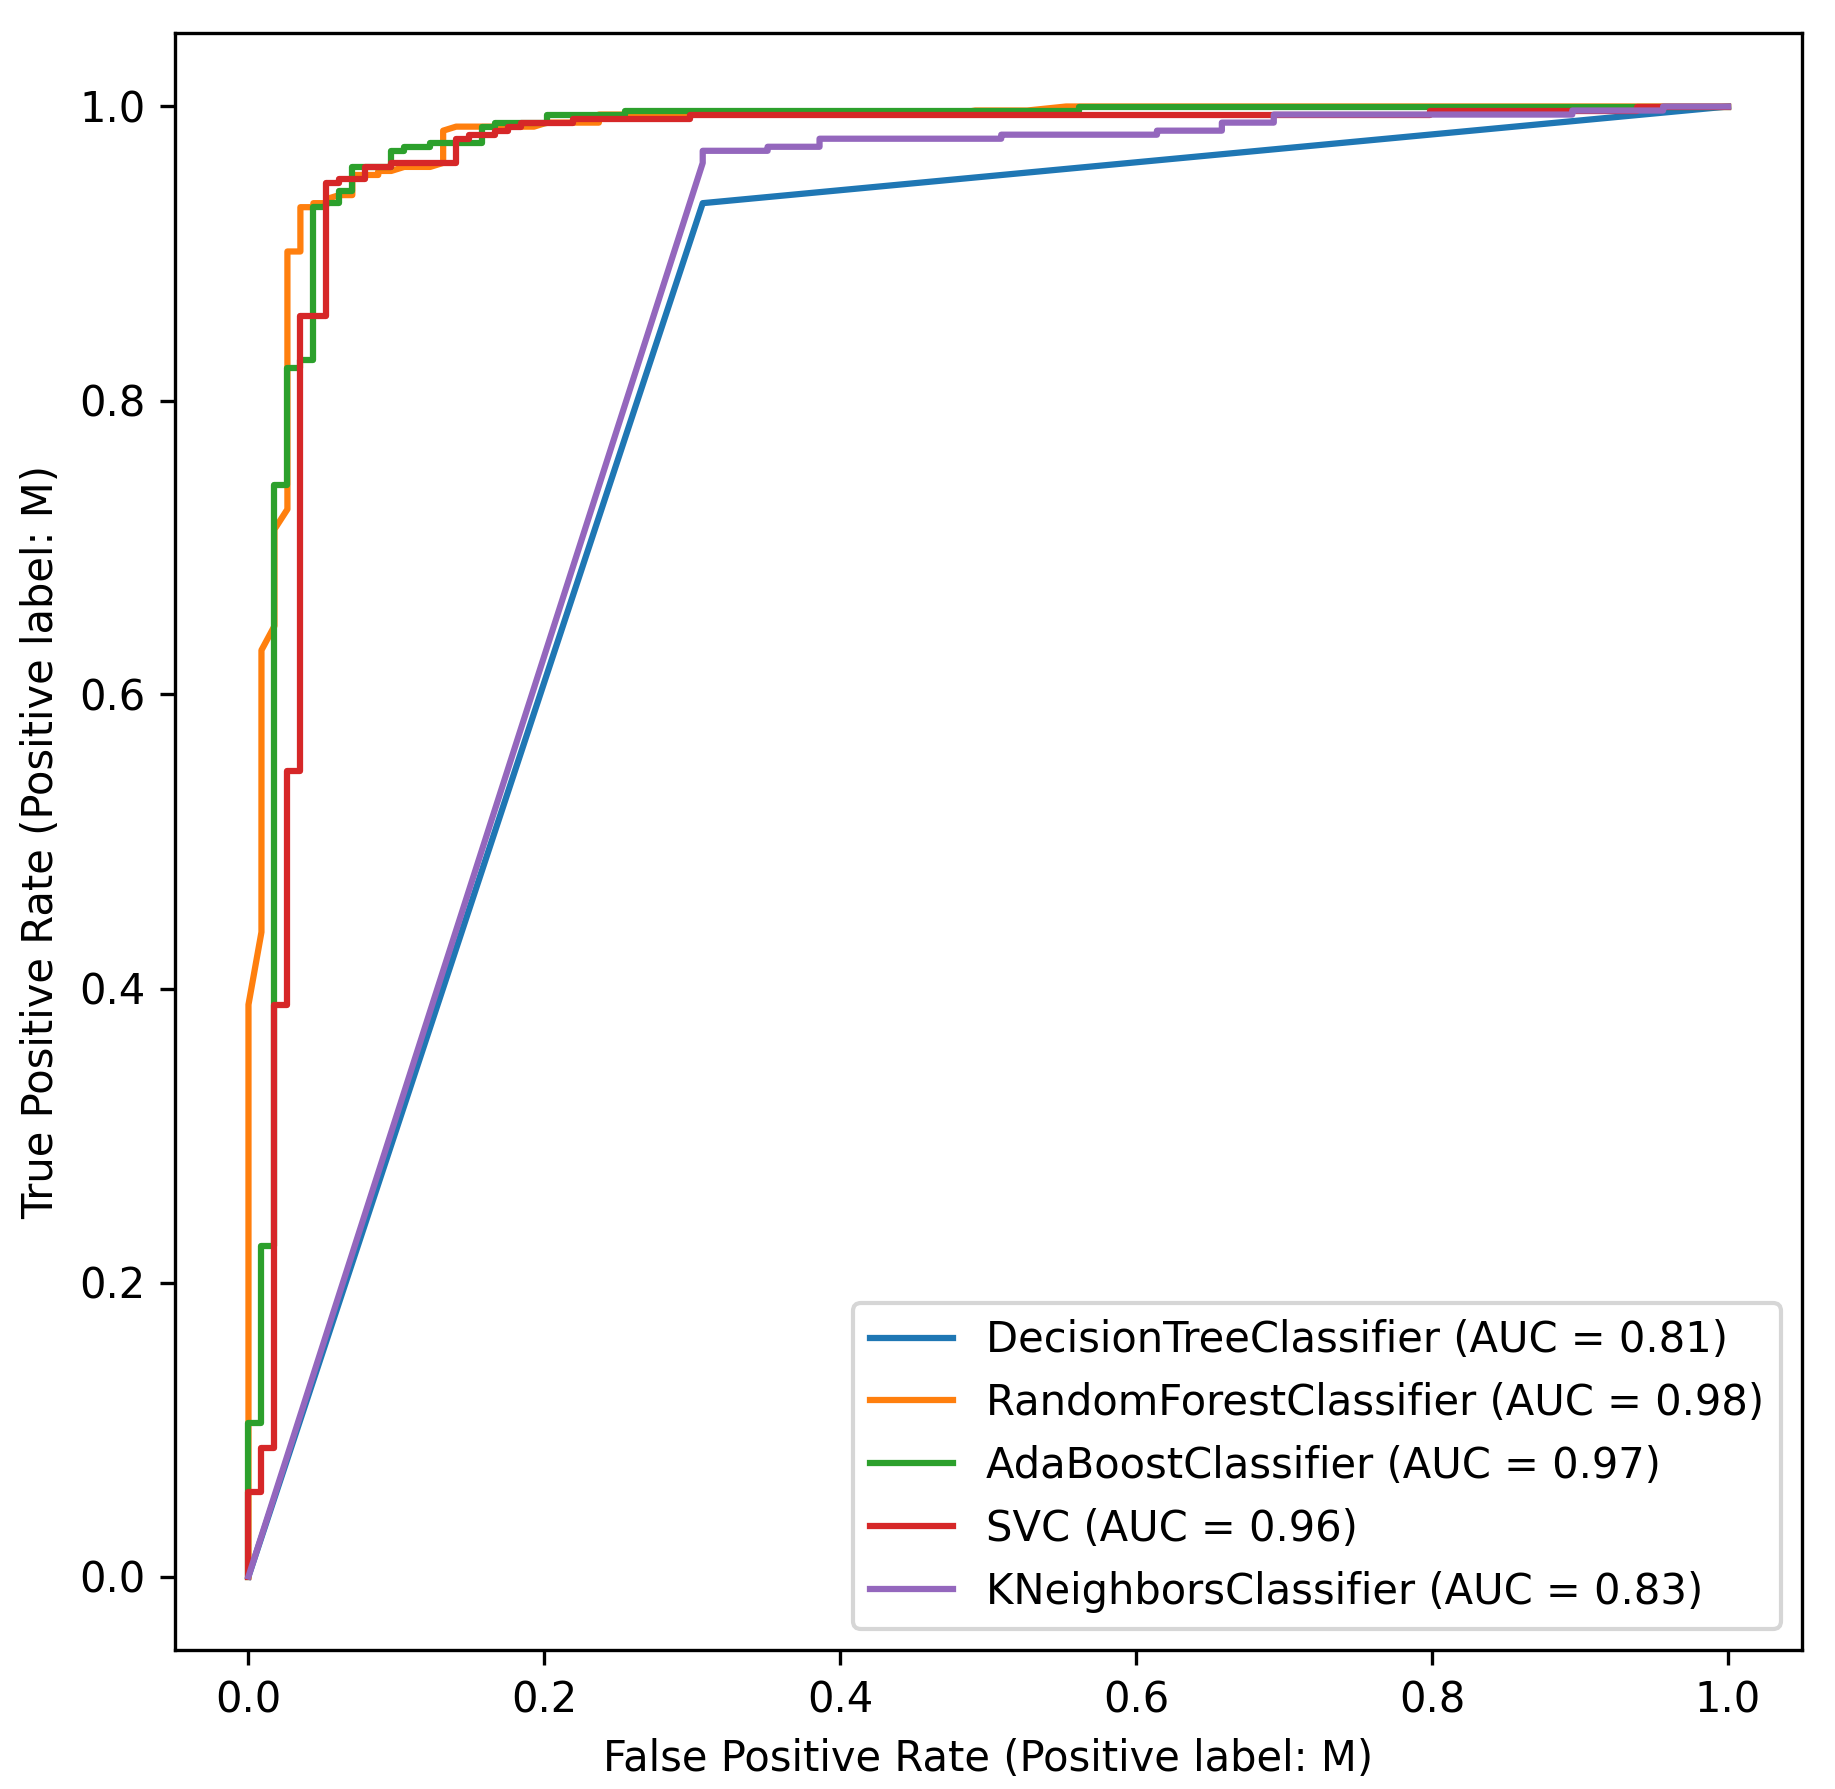
\includegraphics[scale=0.48]{plots/DOC2VEC.png} \\
    \caption{Roc Curve for Doc2Vec}
    \label{fig:rocCurveDoc}
\end{figure}


\section{Conclusion}
In this research report, the printable strings from executable files were analyzed using NLP and ML techniques on a dataset consisting of 2397 samples. The proposed method was successful in accurately classifying an executable as ransomware or benign in a short period of time. The best classifier is a decision tree with the TF-IDF pre-processing NLP technique, providing an accuracy of 99.38\% and a prediction time of 0.0366ms per sample. Not only demonstrate that it is accurate, but also extremely fast. Dynamic analysis techniques, on the other hand, are too time-consuming to be practical in a real-world system; therefore, an accurate static analysis technique is much better suited to a system that aims to be deployed in the real world for real-time detection. A more in-depth analysis of the impact of the types of strings that are used was not explored; instead, all strings were considered in the same form in which they were extracted. Furthermore, the effects of executable compression on the accuracy of the system were not explored. Therefore, future work would evaluate the proposed technique on a dataset of greater size, which would provide a more accurate analysis of the underlying merit. In addition, testing the technique on compressed executables and an analysis of the ideal types of strings to consider would also be beneficial. The proposed technique shows great promise as a method that can be used to quickly provide meaningful insights into whether an executable file contains ransomware.


% Summary of RL extension results
The reinforcement-learning extension described in Section~\ref{sec:rl} (behavioural cloning from the best supervised model followed by REINFORCE fine-tuning) produced a test policy with accuracy 0.93 and macro F1 0.93. These results are reported to demonstrate feasibility of policy bootstrapping and continual adaptation; supervised TF-IDF classifiers still achieve the highest static performance in our experiments, but RL offers a path for online refinement under realistic deployment constraints.

\bibliographystyle{ieeetr}

\bibliography{bibliography.bib}

\end{document}
